\section{Bilder}
\begin{figure}[H]
    \centering
    \caption{Mockup der Übersicht}\label{fig:MockupOverview}
    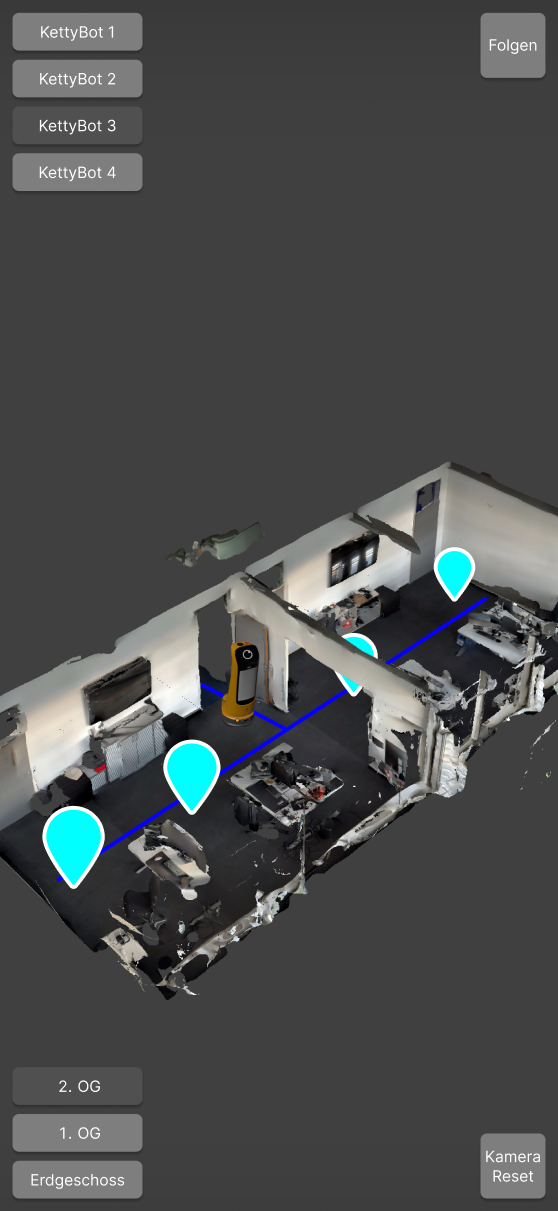
\includegraphics[width=0.5\textwidth]{Mockup Uebersicht}
\end{figure}

\begin{figure}[H]
    \centering
    \caption{Mockup der Steuerung}\label{fig:MockupControls}
    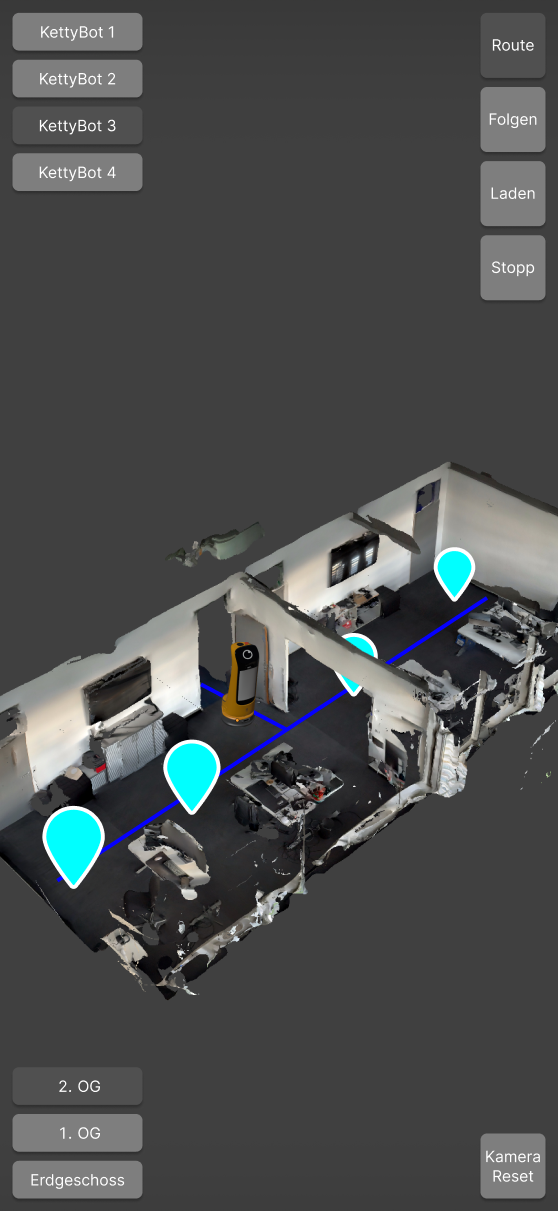
\includegraphics[width=0.5\textwidth]{Mockup Steuerung}
\end{figure}

\begin{figure}[H]
    \centering
    \caption{Mockup des Routenplanungs-Popup}\label{fig:MockupRoutePlanner}
    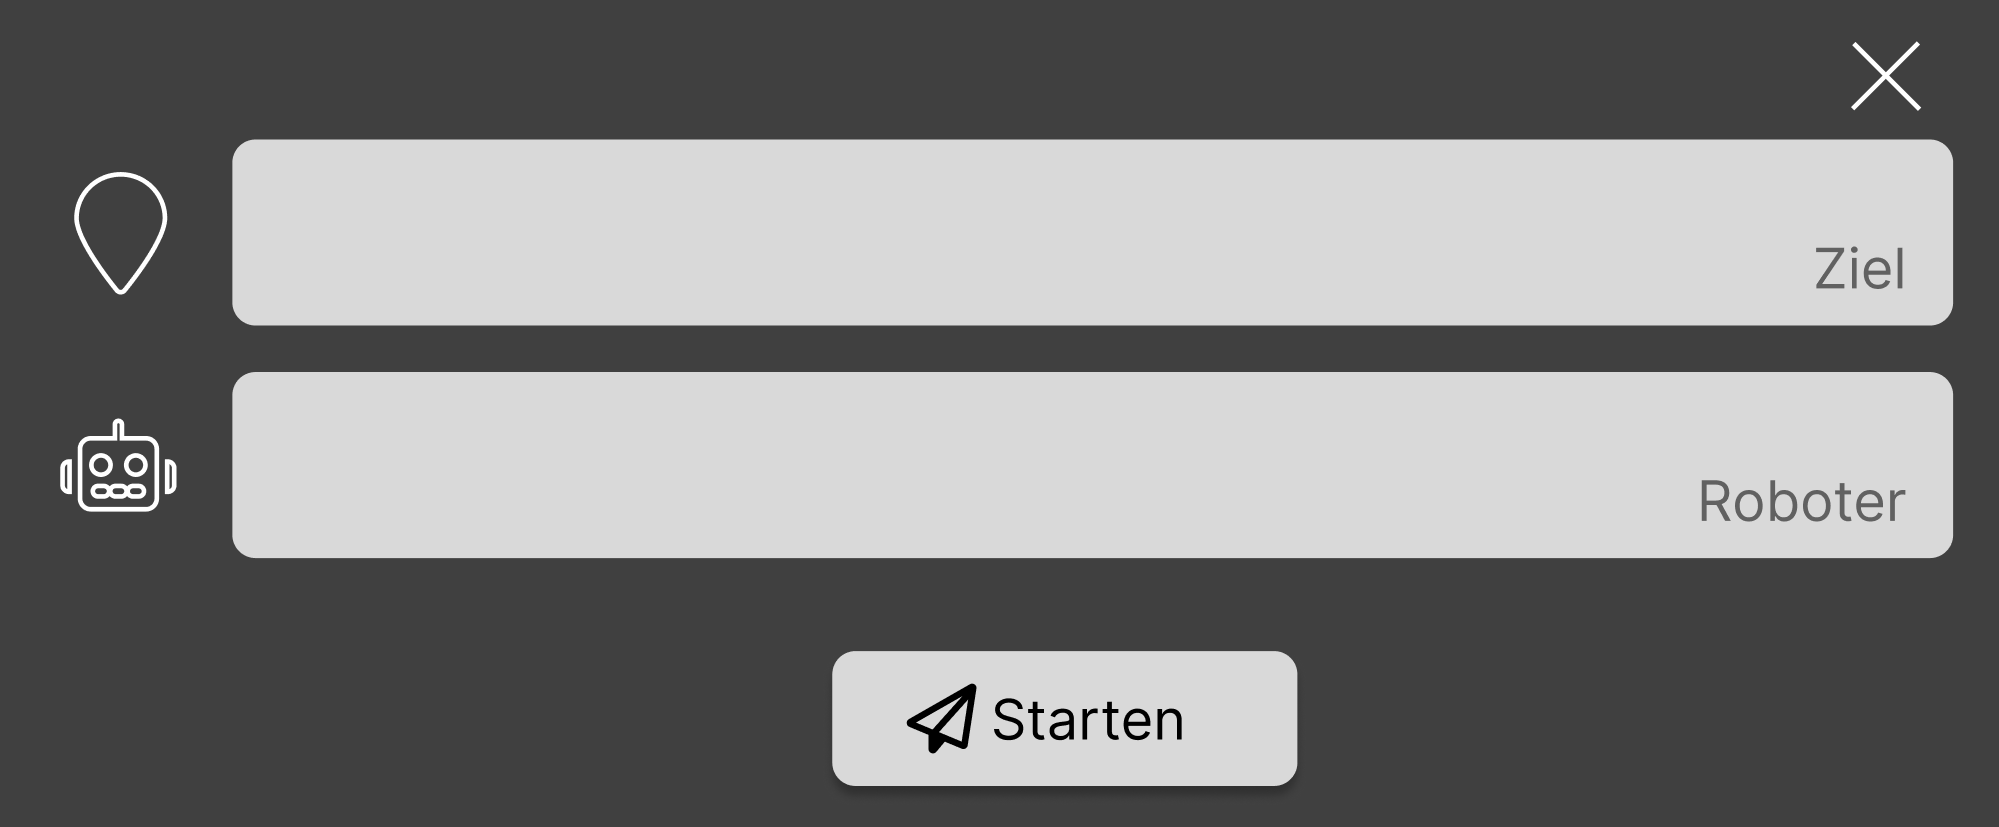
\includegraphics[width=0.9\textwidth]{Mockup Routenplaner}
\end{figure}

\begin{figure}[H]
    \centering
    \caption{Mockup der Verwaltung}\label{fig:MockupAdministration}
    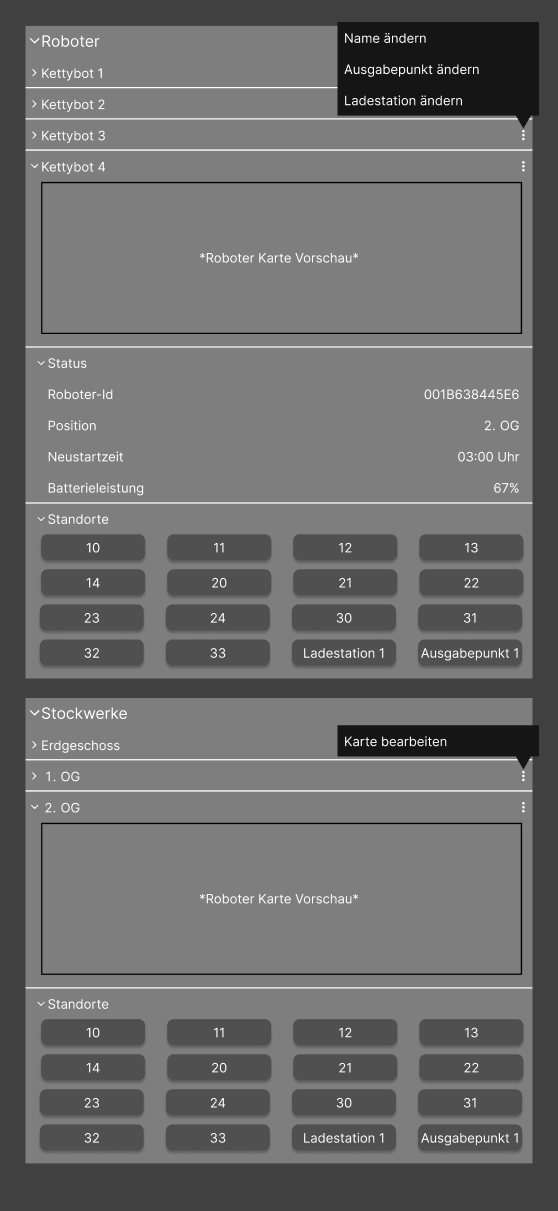
\includegraphics[width=0.5\textwidth]{Mockup Verwaltung}
\end{figure}

\section{Tabellen}
\begin{table}[H]
    \caption{Beschreibung der Probleme in erster Usability Testrunde}\label{tbl:1stUsabilityTestsProblemsDesc}
    \begin{tabular}{l|l}
        Problem Nr. & Beschreibung \\ \hline
        1           & \multicolumn{1}{p{12cm}}{Der Ladestations-Button wurde mit dem Akkustand verwechselt.} \\ \hline
        2           & \multicolumn{1}{p{12cm}}{Die Icons der Buttons sind nicht selbsterklärend. Ohne Anklicken der Buttons kennt man die Funktionen nicht.} \\ \hline
        3           & \multicolumn{1}{p{12cm}}{Die Anordnung der Ergebnisse im Input Dropdown suggeriert, dass man nur nach Nummern und nicht nach Namen suchen kann.} \\ \hline
        4           & \multicolumn{1}{p{12cm}}{Die Tooltips auf der Karte sind durch die Farbwahl schlecht lesbar.} \\ \hline
        5           & \multicolumn{1}{p{12cm}}{Die Fehlermeldungen erklären das Problem nicht.} \\ \hline
        6           & \multicolumn{1}{p{12cm}}{Es wurde versucht, die Modelle in der Übersicht zu verschieben, statt in den Editiermodus zu wechseln.} \\ \hline
        7           & \multicolumn{1}{p{12cm}}{Die Erklärung der Steuerung im Editiermodus ist nicht eindeutig genug.} \\ \hline
        8           & \multicolumn{1}{p{12cm}}{Ohne Loslassen der Maus, kann nicht zwischen Verschieben und Rotieren des Modells gewechselt werden.} \\ \hline
        9           & \multicolumn{1}{p{12cm}}{Es wurde erwartet, dass man in der Routenplanung mehrere Ziele einstellen kann.} \\ \hline
        10          & \multicolumn{1}{p{12cm}}{Es wurde erwartet, dass die Ladestation in der Routenplanung eingestellt werden kann.} \\ \hline
        11          & \multicolumn{1}{p{12cm}}{Der Toast Dialog, der die Steuerung im Editiermodus erklärt, wurde nicht angezeigt.} \\ \hline
        12          & \multicolumn{1}{p{12cm}}{Es gab Unklarheit darüber, wohin das 3D-Modell verschoben werden muss.} \\ \hline
        13          & \multicolumn{1}{p{12cm}}{Die Darstellung der 3D-Modelle sieht kaputt aus.} \\ \hline
        14          & \multicolumn{1}{p{12cm}}{Ein Stockwerk-Button wird durch das Beta Modus Tag von chayns verdeckt.} \\ \hline
        15          & \multicolumn{1}{p{12cm}}{Beim Positionieren des Modells gab es Schwierigkeiten.} \\ \hline
        16          & \multicolumn{1}{p{12cm}}{Der Roboter wurde aufgrund des Icons – das über diesem angezeigt wird – nicht erkannt.} \\ \hline
        17          & \multicolumn{1}{p{12cm}}{Die Transparenz der Lieferauftrag-Fläche macht Texte schlecht lesbar und sieht insgesamt nicht gut aus.} \\ \hline
        18          & \multicolumn{1}{p{12cm}}{Die Robotersteuerungs-Buttons werden nicht angezeigt, wenn die Routenplanung geöffnet ist.} \\ \hline
        19          & \multicolumn{1}{p{12cm}}{Es wurde erwartet, dass man nach dem Schließen des Editiermodus wieder im Nutzermodus landet.} \\ \hline
        20          & \multicolumn{1}{p{12cm}}{Der Button zum Zurücksetzen der Kameraposition wurde im Editiermodus nicht gefunden, da dieser an einer anderen Position als in der Übersicht angezeigt wird.} \\
    \end{tabular}
\end{table}
\begin{table}[H]
    \caption{Beschreibung der Probleme in zweiter Usability Testrunde}\label{tbl:2ndUsabilityTestsProblemsDesc}
    \begin{tabular}{l|l}
        Problem Nr. & Beschreibung \\ \hline
        1           & \multicolumn{1}{p{12cm}}{Es gab Unklarheit darüber wie man die Karte rotiert.} \\ \hline
        2           & \multicolumn{1}{p{12cm}}{Beim Entfernen einer Roboterauswahl wird in das Stockwerk des Roboters gewechselt, obwohl das nur bei der Auswahl eines Roboters passieren sollte.} \\ \hline
        3           & \multicolumn{1}{p{12cm}}{Es wurde erwartet, dass man den Roboter über das Ladestations-Icon auf der Karte zur Ladestation schicken kann.} \\ \hline
        4           & \multicolumn{1}{p{12cm}}{Die Suchfunktion zum Auswählen eines Standorts wurde nicht gefunden, da das Routenplanungs-Popup nicht geöffnet wurde.} \\ \hline
        5           & \multicolumn{1}{p{12cm}}{Es gab Irritation darüber, dass die Steuerung über einen Tooltip erklärt wird.} \\ \hline
        6           & \multicolumn{1}{p{12cm}}{Der Editiermodus wurde nicht im Nutzermodus gefunden, da das Icon des Buttons falsch verstanden wurde.} \\ \hline
        7           & \multicolumn{1}{p{12cm}}{Der Editiermodus wurde nicht im Admin-Modus gefunden, da das Kontextmenü übersehen wurde.}
    \end{tabular}
\end{table}
